\documentclass[12pt,a4paper]{article}
\usepackage[left=25mm,right=25mm,top=25mm,bottom=25mm]{geometry} %Margins
\usepackage[utf8]{inputenc} % Required for inputting international characters
\usepackage[T1]{fontenc} % Output font encoding for international characters
\usepackage[dvipsnames]{xcolor}
\usepackage{graphicx} % Insert images
\usepackage{enumitem} % List with letters
\usepackage{fancyhdr} % Headers and footers
\usepackage[colorlinks = true,
            linkcolor = blue,
            urlcolor  = blue,
            citecolor = blue,
            anchorcolor = blue]{hyperref} % Clickable table of content
%\usepackage{sectsty} % Change the headings
%\usepackage{titlesec} % Remove numbers of the sections
\usepackage{amsmath}
\usepackage{centernot} %center not on maths sign
\usepackage{tikz}
\usetikzlibrary{calc}
%\usepackage{fontspec}
%\setmainfont{Calibri}
\usepackage{mathtools}
\DeclarePairedDelimiter\ceil{\lceil}{\rceil}
\DeclarePairedDelimiter\floor{\lfloor}{\rfloor}

\usepackage{float}
\usepackage{colortbl}
\usepackage{amsfonts}
\setlength\parindent{0pt}
\pagestyle{fancy}
\fancyhf{}
\rhead{\today} % Right header
\lhead{Fradet \& Larrouy} % Left header
\chead{Lab 3} % Center header
\rfoot{Page \thepage} % Right footer

\hypersetup{
    colorlinks=true, %set true if you want colored links
    linktoc=all,     %set to all if you want both sections and subsections linked
    linkcolor=Blue,  %choose some color if you want links to stand out
}

\usepackage{listings}

% Python style for highlighting
\newcommand\pythonstyle{\lstset{
language=Python,
basicstyle=\ttm,
otherkeywords={self},             % Add keywords here
keywordstyle=\ttb\color{ForestGreen},
emph={MyClass,__init__},          % Custom highlighting
emphstyle=\ttb\color{blue},    % Custom highlighting style
stringstyle=\color{RedViolet},
frame=tb,                         % Any extra options here
showstringspaces=false            % 
}}

\lstnewenvironment{python}[1][]
{
\pythonstyle
\lstset{#1}
}
{}

\newcommand\pythonexternal[2][]{{
\pythonstyle
\lstinputlisting[#1]{#2}}}

\begin{document}

%----------------------------------------------------------------------------------------
%	TITLE PAGE
%----------------------------------------------------------------------------------------

\begin{titlepage} % Suppresses headers and footers on the title page
	
	\vspace{4\baselineskip} % Whitespace below ESILV logo

	\centering % Center everything on the title page

	\textcolor{White}{ADSA-4A-IBO\\} % Workshop title
	
	\vspace{0.5\baselineskip} % Whitespace above workshop number
	\textcolor{White}{W[3]\\}	
	\vspace{2\baselineskip} % Whitespace above horizontal rule
	
	%------------------------------------------------
	%	Title
	%------------------------------------------------
	
	\rule{\textwidth}{1.6pt}\vspace*{-\baselineskip}\vspace*{2pt} % Thick horizontal rule
	\rule{\textwidth}{0.4pt} % Thin horizontal rule
	
	\vspace{0.75\baselineskip} % Whitespace above the title
	
	\textcolor{Blue}{\Large Big Data Frameworks} % Title
	\vspace{0.75\baselineskip}
	\textcolor{Blue}{\large \\Stream Processing and Messaging using Apache SPARK} % Workshop title
	
	\vspace{0.75\baselineskip} % Whitespace below the title
	
	\rule{\textwidth}{0.4pt}\vspace*{-\baselineskip}\vspace{3.2pt} % Thin horizontal rule
	\rule{\textwidth}{1.6pt} % Thick horizontal rule
	
	\vspace{2\baselineskip} % Whitespace after the title block
	
	%------------------------------------------------
	%	Authors
	%------------------------------------------------	
	
	Authors
	
	\vspace{0.5\baselineskip} % Whitespace before the editors
	
	Guillaume Fradet \\ Félix Larrouy \\% Editor list
	
	\vspace{2\baselineskip} % Whitespace below the editor list
	
	Project is hosted on github: \href{https://github.com/felixlarrouy/tweets-streaming}{https://github.com/felixlarrouy/tweets-streaming}
	
	\vfill % Whitespace between author names and last modification date
	
	%------------------------------------------------
	%	Last modification date
	%------------------------------------------------
	
	\today

\end{titlepage}

%------------------------------------------------
%	Summary
%------------------------------------------------

\renewcommand{\contentsname}{Summary}
\tableofcontents

\newpage

\section{Server side}

Here is the code of our \textbf{server.py} file.\\

\pythonexternal{server.py} 

\textcolor{White}{aaaaaa}

We used the \textbf{Tweepy} library, which is a Twitter client for Python. First, we need to store our Twitter developper account credentials. Then, we created a \textbf{TweetsListener} class which will be handling the streaming of tweets. The most important method here is \textit{on\_data}, which receives the data from Tweeter and send it to a socket object. We get each tweet in a JSON format and only send the \textit{'text'} value to the socket.\\

Next we connect to tweeter streaming with the function \textit{sendData}. We set the authorizations with our credentials and collect every tweet containing \textit{sys.argv[1]} (which is a \textit{string}).\\

Finally, we will create a socket object and start the streaming process. We bind the socket to a reserved localhost port, wait for a client connection, connect to the client, and send data to the client.\\

We are now ready to receive the tweets from the client side.

\section{Client side}

\pythonexternal{client.py} 

\textcolor{White}{aaaaaa}

We create a \textit{socketTextStream}, where we expect a Twitter streaming connection on the same port as the one specified in the server side. Next we create a \textit{DStream} where we specify the window duration, which has to be a multiple of the batch duration.\\

Next we do some transformations on the \textit{DStream} to count the words where there is a '\#' as the first character.\\

Then for each RDD of the \textit{DStream}, we we store the RDD as a temporary SQL table thanks to the \textit{SQLContext} instance of our \textit{DStream}. We can then query the temporary table which as been created to get the most popular tweets in the window, store the results in a dataframe and plot the hastags.\\

We are now ready to start the streaming process. Top hashtags will be displayed every \textit{window\_duration} seconds.

\section{Usage}

The first thing we need to do is to launch our server. 

To do so, we run the python file \emph{server.py} with a word (or chain of words) as argument. This argument is a condition on the tweets that we will stream, such that all tweets content must include our word(s).
\\

\emph{Example: if the argument is "Messi", we will get all the tweets containing "Messi".}
\\

\begin{figure}[h]
    \centering
    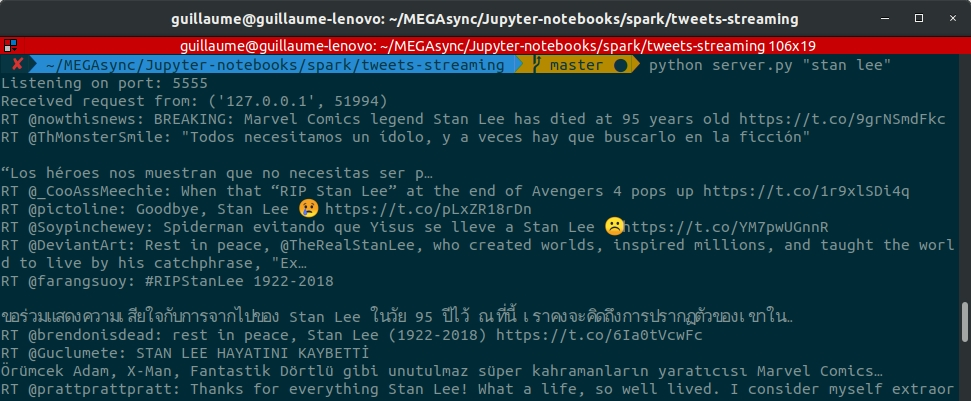
\includegraphics[width=1.0\textwidth]{usage-server.jpg}
    \caption{Launch the server to stream the tweets containing "Stan Lee"}
    \label{fig:my_label}
\end{figure}

Then we can launch the client code in a Jupyter notebook to perform the spark operations on the tweets. \\

\begin{figure}[H]
    \centering
    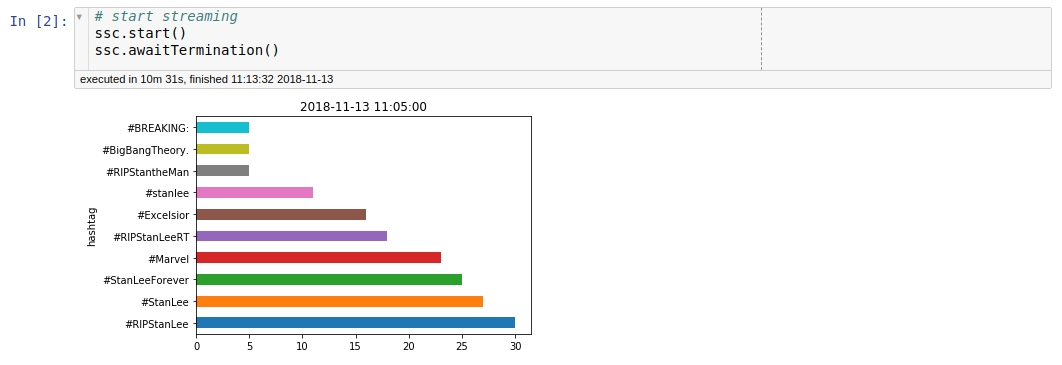
\includegraphics[width=1.0\textwidth]{usage-client.jpg}
    \caption{Start the pyspark streaming in a Jupyter notebook}
    \label{fig:my_label}
\end{figure}

\newpage
\section{Outputs}

We streamed tweet containing "stan lee", for window durations of 30 seconds, 1 minute, and 5 minutes. Here are the results we got.

\begin{figure}[H]
    \centering
    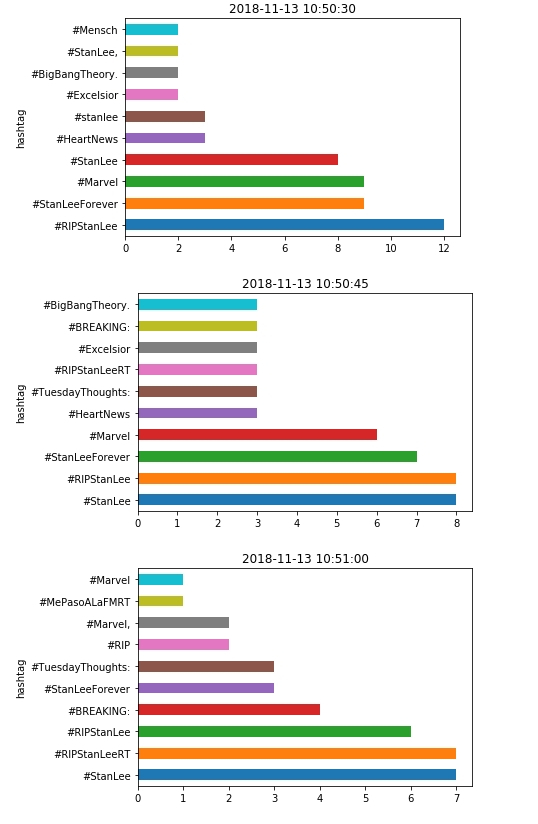
\includegraphics[width=12cm]{ouput1-30sec.jpg}
    \caption{Batch duration of 15 seconds, window duration of 30 seconds}
    \label{fig:my_label}
\end{figure}

\begin{figure}[h]
    \centering
    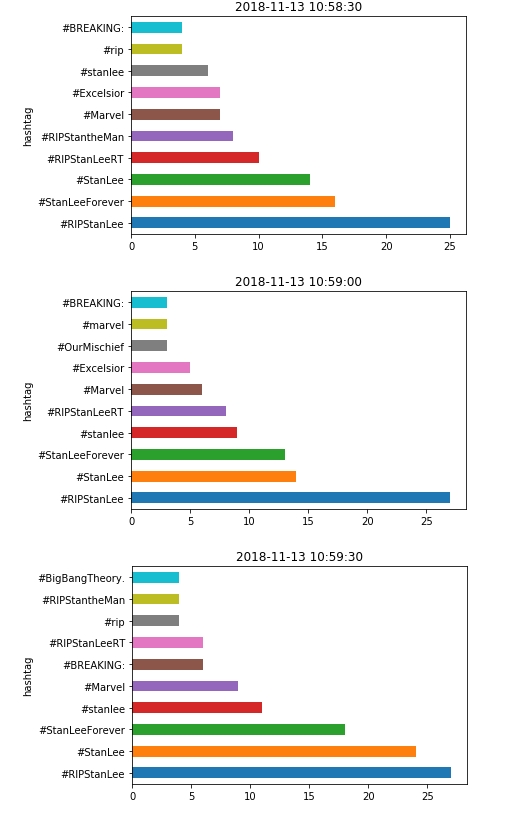
\includegraphics[width=12cm]{output2-1min.jpg}
    \caption{Batch duration of 30 seconds, window duration of 1 minute}
    \label{fig:my_label}
\end{figure}

\begin{figure}[h]
    \centering
    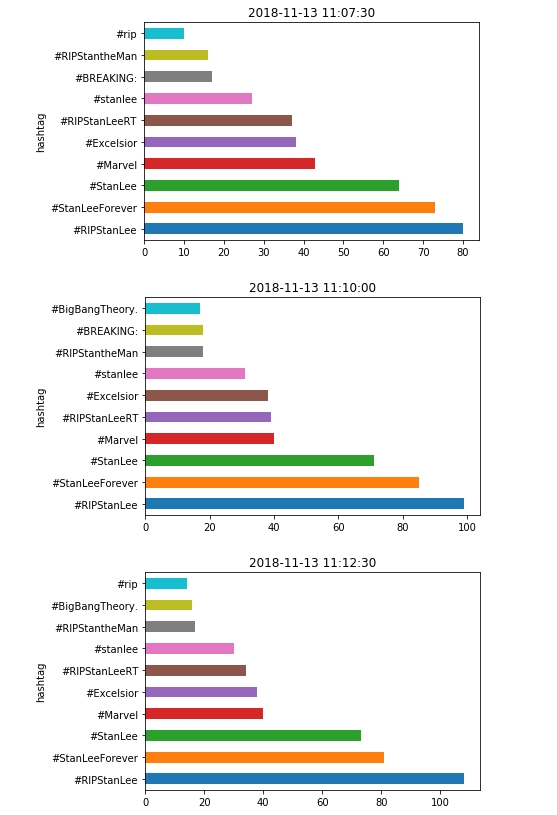
\includegraphics[width=12cm]{output3-5min.jpg}
    \caption{Batch duration of 2 minutes 30 seconds, window duration of 5 minutes}
    \label{fig:my_label}
\end{figure}

\end{document}
